\documentclass[a4paper]{article}
\usepackage[UTF8]{ctex}

\headheight 0.5cm
\textheight 23.5cm \textwidth 15.8cm
\topmargin -1.5cm \oddsidemargin 0.3cm \evensidemargin -0.3cm

\usepackage{fancyhdr}
\usepackage{float}
\usepackage{graphicx}
\usepackage{amssymb}
\usepackage{amsmath}
\usepackage{amsthm}

\newtheorem{theorem}{Thm}
\newtheorem*{definition}{Def}
\newtheorem{lemma}{Lemma}
\newtheorem{corollary}{Cor}

\pagestyle{fancy}

\title{B 样条简介}
\author{Litt Phia}


\begin{document}
\maketitle
\tableofcontents

\clearpage
\section{样条函数}

\begin{definition}[样条函数]
    样条函数是由具有某些连续性条件的一些子区间上的多项式构成的分段多项式。
\end{definition}

\begin{definition}[$k$ 次样条函数]
    给定结点 $t_0 < t_1 < \cdots < t_n$,将满足下列条件的函数 $\mathcal{S}$ 称为 $t_0,\ t_1,\ \cdots,\ t_n$ 上的一个 $k$ 次样条函数:
    \begin{itemize}
        \item[1] 在每一个区间 $[t_{i - 1},\ t_{i})$ 上,$S$ 是一个次数 $\leqslant k$ 的多项式
        \item[2] 在 $[t_0,\ t_n]$ 上 $S$ 有 $(k - 1)$ 阶连续导数。
    \end{itemize}
\end{definition}
    \noindent 因此 $\mathcal{S}$ 是一个次数至多是 $k$ 次的分段多项式,并且具有直到 $k - 1$ 阶的连续导数。

    取实轴上一组结点序列 $\{t_i\}$。为了便于理论上的讨论,我们将结点集合左端拓展到 $-\infty$,右端拓展到 $+\infty$,使其成为一个无限集:
    \begin{gather*}
        \cdots < t_{-2} < t_{-1} < t_{0} < t_{1} < t_{2} < \cdots
    \end{gather*}

    在之后的讨论中,我们假设这个结点序列是固定的,并在此基础上建立所有的样条。


\section{B 样条的定义}

    \noindent 一般将零次 B 样条记为 $B_i^0$,图形如下所示。
    \begin{figure}[H]
        \centering
        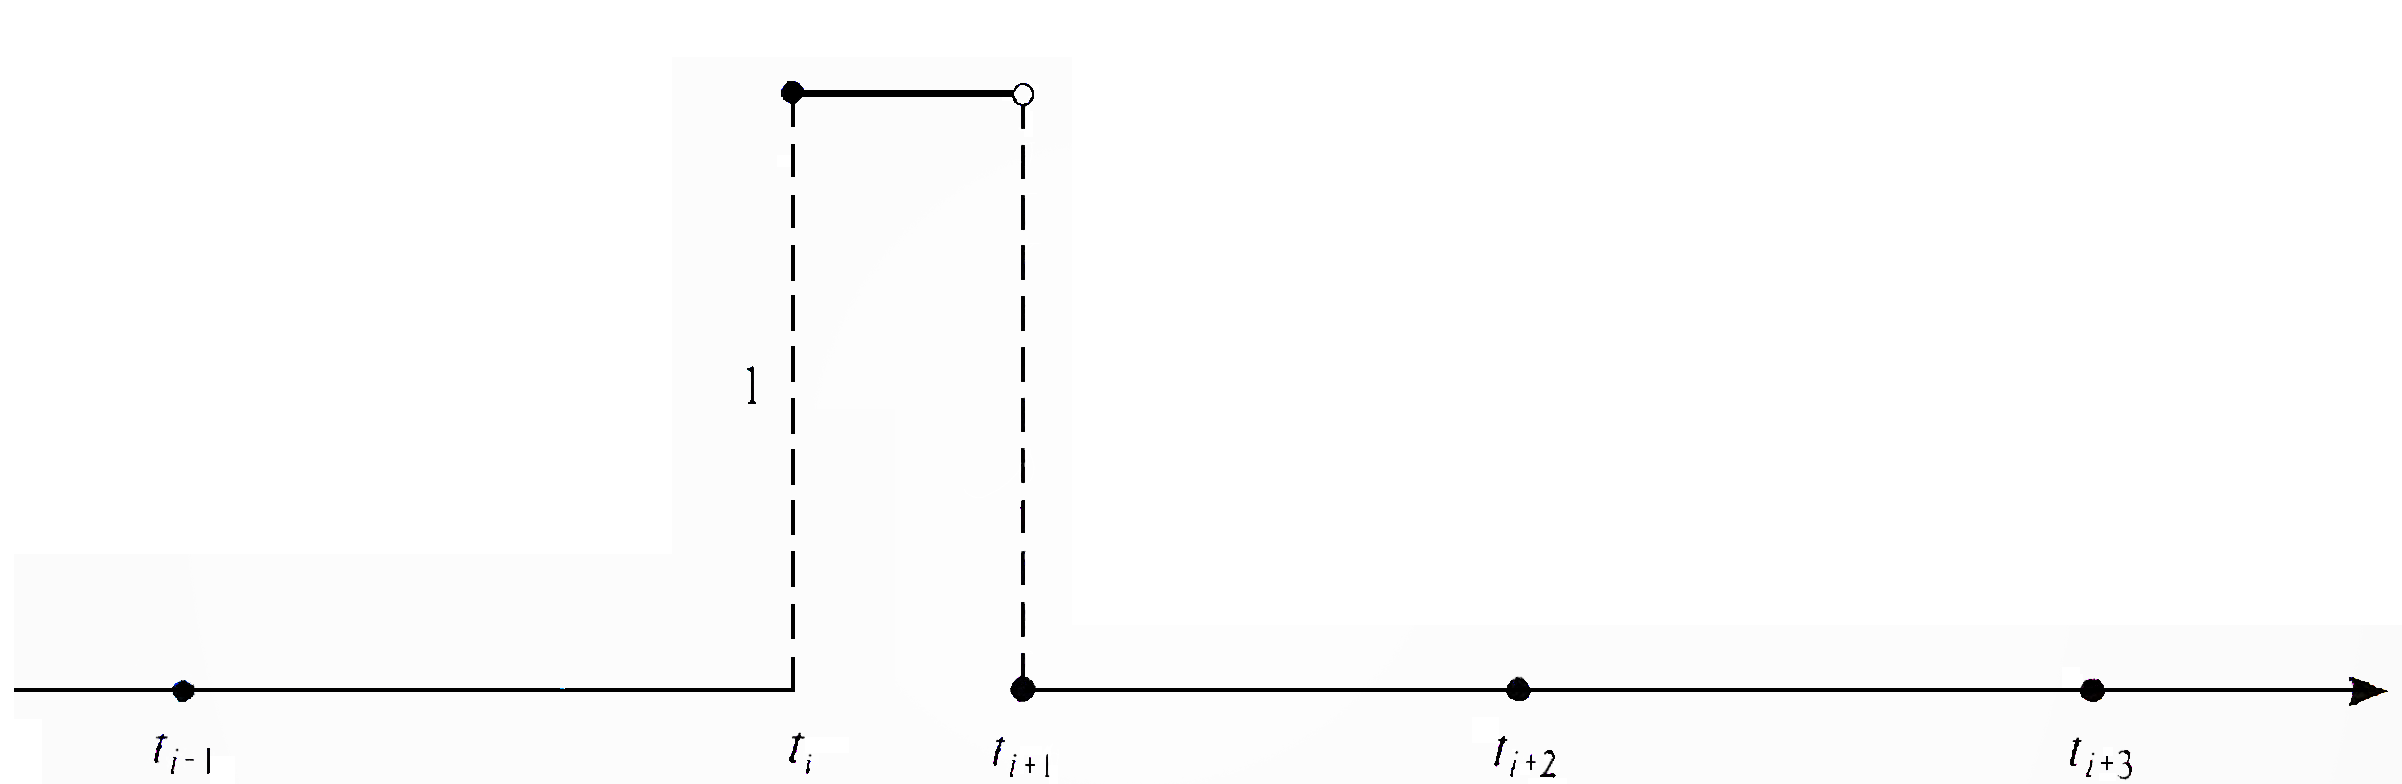
\includegraphics[width = 12cm, height = 4cm]{0-order-BSpline.png}
    \end{figure}

    \noindent 指标 $i$ 取遍全体正数。深色圆点表明我们定义 $B_i^0(t_{i}) = 1$ 以及 $B_i^0(t_{i+1}) = 0$。正式的定义是:
    \begin{equation}
        \label{definition-0-B-Spline}
        B_i^0(x) = \left\{\begin{aligned}
            &1 \qquad t_{i} \leqslant x < t_{i+1} \\
            &0 \qquad otherwise
      \end{aligned}\right.
    \end{equation}

    这些 B 样条构成一个无穷序列 $\{B_i^0:i\in \mathbb{Z}\}$。可以看出它们的一些显而易见的性质:
    \begin{itemize}
        \item 使得 $B_i^0 \neq 0$ 的集合定义为 $B_i^0$ 的支撑,为区间 $[t_{i},\ t_{i+1})$
        \item 对一切 $i$ 及 $x$,$B_i^0(x) \geqslant 0$
        \item 在整个实轴上 $B_i^0(x)$ 是右连续的
        \item 对一切 $x5$,$\displaystyle\sum_{i = -\infty}^{\infty} B_i^0(x) = 1$
    \end{itemize}

    注意到对于给定结点序列上的全体零次样条,假设我们标准化这些样条使其都是右连续的,那么样条 $B_i^0$ 构成这些结点上全体零次样条的 Schauder 意义下的一组基。
    
    \begin{definition}[高次 B 样条]
        定义 $k$ 次 B 样条
        \begin{equation}
            B_i^k (x) = \left(\frac{x - t_i}{t_{i+k} - t_{i}}\right) B_{i}^{k-1}(x) + \left(\frac{t_{i+k+1} - x}{t_{i+k+1} - t_{i+1}}\right) B_{i+1}^{k-1}(x) \qquad (k \geqslant 1)
        \end{equation}

        \noindent 引入线性函数
        \begin{equation}
            V_i^k (x) = \frac{x - t_i}{t_{i+k} - t_{i}}
        \end{equation}

        \noindent 那么上述递归定义式可写为
        \begin{equation}
            \label{definition-k-B-Spline}
            B_i^k = V_i^k B_{i}^{k-1} + (1 - V_{i+1}^k) B_{i+1}^{k-1}
        \end{equation}
    \end{definition}

    由定义易见 $B_i^k$ 是一个次数 $\leqslant k$ 的分段多项式。借助上式可以给出 $B_i^1(x)$ 的显式公式如下:
    \begin{equation}
    \label{expression-1-B-Spline}
        B_i^1(x) = \left(\frac{x - t_i}{t_{i+1} - t_{i}}\right) B_i^0(x) + \left(\frac{t_{i+2} - x}{t_{i+2} - t_{i+1}}\right) B_{i+1}^0(x)
        = \left\{\begin{aligned}
            & \frac{x - t_i}{t_{i+1} - t_{i}} \quad\qquad t_{i} \leqslant x < t_{i+1} \\
            & \frac{t_{i+2} - x}{t_{i+2} - t_{i+1}} \qquad t_{i+1} \leqslant x < t_{i+2} \\
            & \qquad 0 \qquad\qquad otherwise
        \end{aligned}\right.
    \end{equation}
    其图形如下所示
    \begin{figure}[H]
        \centering
        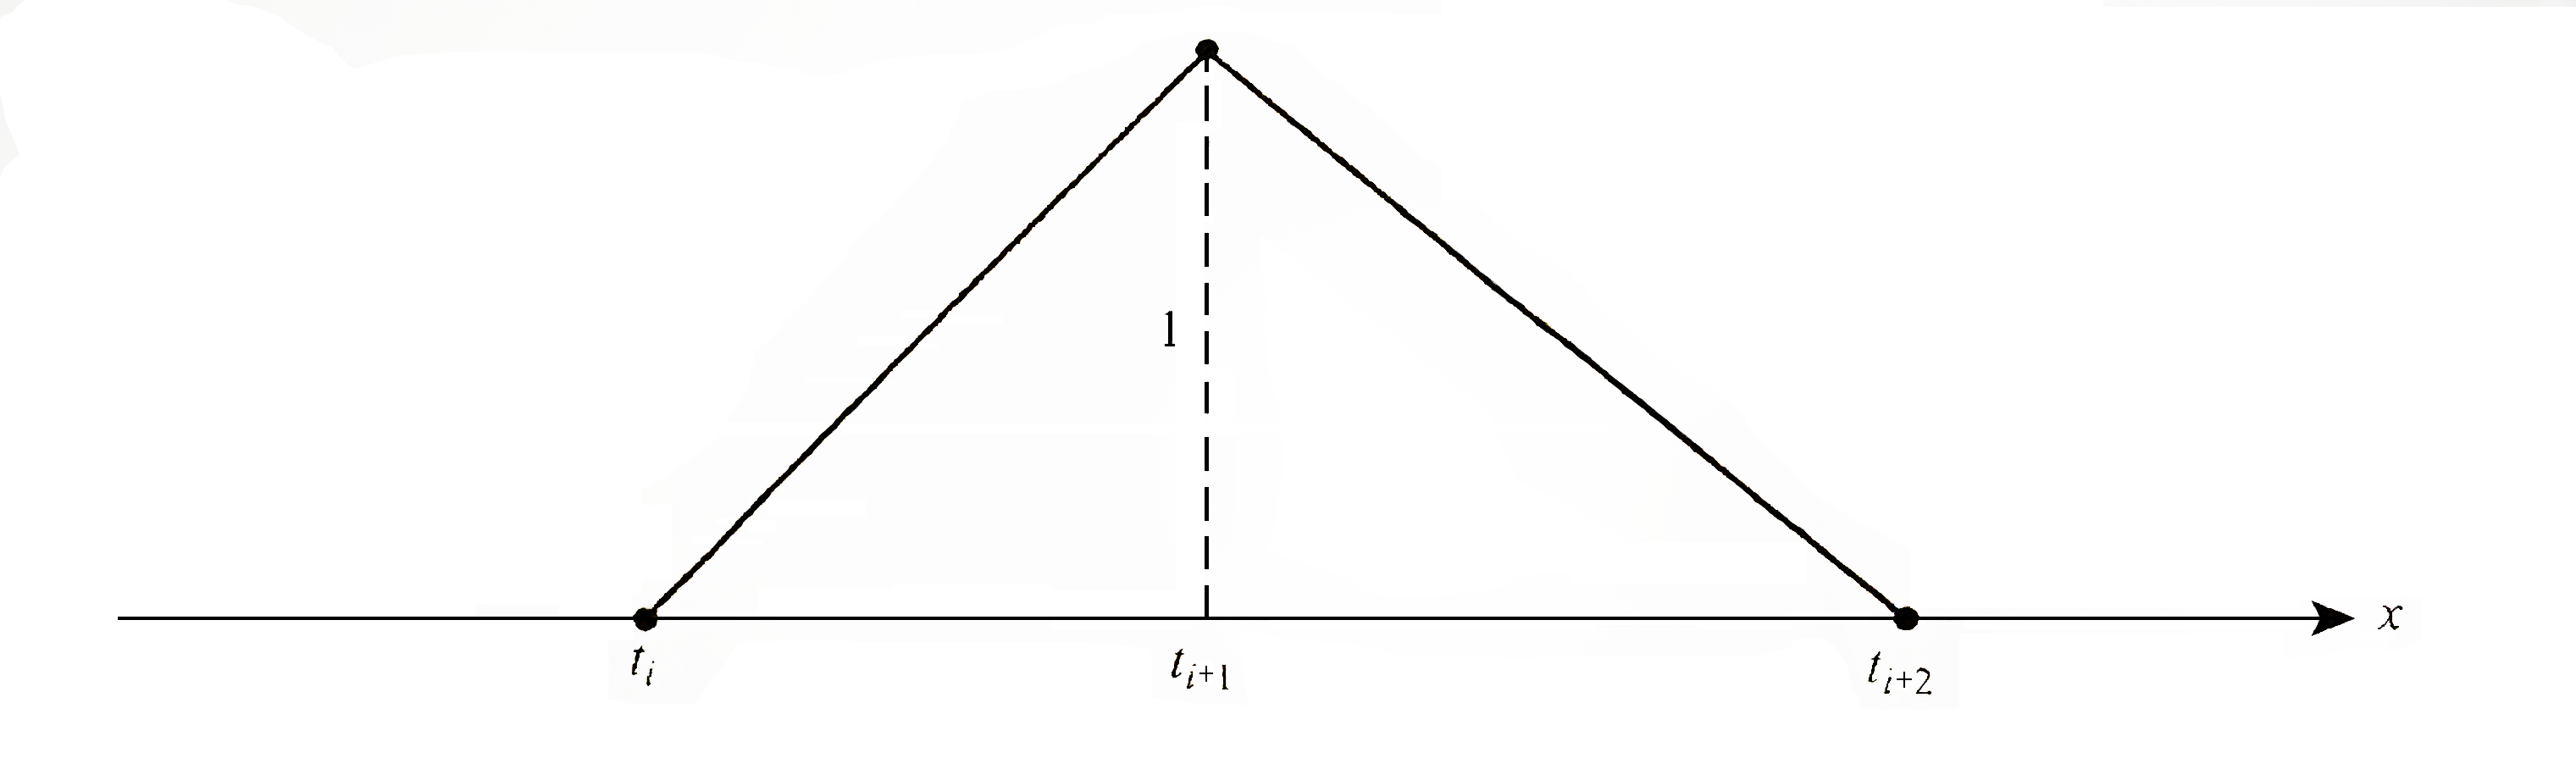
\includegraphics[width = 12cm, height = 4cm]{1-order-BSpline.png}
    \end{figure}

    \noindent 此外可以看出 $B_i^1$ 的性质:
    \begin{itemize}
        \item $B_i^1 \neq 0$ 的支撑是 $(t_{i},\ t_{i+1})$
        \item 对一切 $i$ 及 $x$,$B_i^1(x) \geqslant 0$
        \item $B_i^1(x)$ 连续并且在除点 $t_{i}$,$t_{i+1}$,$t_{i+2}$ 之外的每一点可微
        \item 对一切 $x$,$\displaystyle\sum_{i = -\infty}^{\infty} B_i^0(x) = 1$
    \end{itemize}

    这里给出最后一个性质的证明:对 $\forall x \in \mathbb{R}$,可以找到指标 $j$ 使得 $t_{j} \leqslant x < t_{j+1}$,因而对于除 $i = j$ 或 $i = j - 1$ 之外的所有 $i$,都有 $B_i^1(x) = 0$,故
    \begin{equation}
        \sum_{i = -\infty}^{\infty} B_i^1(x) = B_{j-1}^1(x) + B_{j}^1(x) = \frac{t_{j+1} - x}{t_{j+1} - t_j} + \frac{x - t_j}{t_{j+1} - t_{j}} = 1
    \end{equation}


\section{B 样条的性质}

\begin{lemma}[B 样条的支撑引理]
\label{lemma-B-Spline-Suppport}
    若 $k \geqslant 1$ 并且 $x \notin (t_{i},\ t_{i+k+1})$,则 $B_i^k(x) = 0$。
\end{lemma}
\begin{proof}[Proof]
    已知对于 $k = 1$ 引理成立,但对于 $k = 0$ 不成立。假设对于某个指标 $k-1$ 上述结论成立,那么若 $x \notin (t_{i},\ t_{i+k+1})$,则 $x \notin (t_i,\ t_{i+k})$ 并且 $x \notin (t_{i+1},\ t_{i+k+1})$,根据归纳假设, $B_{i}^{k-1}(x) = 0$ 且 $B_{i+1}^{k-1}(x) = 0$。由 (\ref{definition-k-B-Spline}) 式知 $B_i^k(x) = 0$ 成立。
\end{proof}

\begin{lemma}[B 样条的正性引理]
\label{lemma-B-Spline-Positive}
    设 $k \geqslant 0$,若 $x \in (t_{i},\ t_{i+k+1})$,则 $B_i^k(x) > 0$。
\end{lemma}
\begin{proof}[Proof]
    已知对于 $k = 0$ 或 $k = 1$ 时引理成立,但对于 $k = 0$ 不成立。假设对于某个指标 $k-1$ 上述结论成立,$k > 1$。那么对于一切 $i$ 和 $x$,根据归纳假设和引理 \ref{lemma-B-Spline-Suppport} 知 $B_i^k(x) \geqslant 0$。设 $t_{i} < x < t_{i+k+1}$,则 (\ref{definition-k-B-Spline}) 右端项的线性因式是正的。再由归纳假设知在 $(t_{i},\ t_{i+k})$ 中 $B_{i}^{k-1}(x) > 0$,在 $(t_{i+1},\ t_{i+k+1})$ 中 $B_{i+1}^{k-1}(x) > 0$,因 $k > 1$,这两个区间相互重叠,由 (\ref{definition-k-B-Spline}) 式可推出 $B_i^k(x) > 0$。
\end{proof}

\begin{lemma}[B 样条的递推关系引理]
\label{lemma-B-Spline-Recursive}
    对一切 $k \geqslant 0$,我们有
    \begin{equation}
        \sum_{i = -\infty}^{\infty} c_i B_i^k = \sum_{i = -\infty}^{\infty} \left[ c_i V_i^k + c_{i-1} (1 - V_i^k) \right] B_{i}^{k-1}
    \end{equation}
    则 $B_i^k(x) > 0$。
\end{lemma}
\begin{proof}[Proof]
    利用 (\ref{definition-k-B-Spline}) 式和基本的级数操作,有:
    \begin{equation}
    \begin{aligned}
        \sum_{i = -\infty}^{\infty} c_i B_i^k & = \sum_{i = -\infty}^{\infty} c_i \left[ V_{i}^{k} B_{i}^{k-1} + (1 - V_{i+1}^{k}) B_{i+1}^{k-1} \right] \\
        & = \sum_{i = -\infty}^{\infty} c_i V_{i}^{k} B_{i}^{k-1} + \sum_{i = -\infty}^{\infty} c_{i-1} (1 - V_{i}^{k}) B_{i}^{k-1} \\
        & = \sum_{i = -\infty}^{\infty} \left[ c_i V_i^k + c_{i-1} (1 - V_i^k) \right] B_{i}^{k-1}
    \end{aligned}
    \end{equation}
\end{proof}


\section{数值计算过程}

    注意到在引理 \ref{lemma-B-Spline-Recursive} 中,系数 $c_i$ 可以是常数或者函数,因此它提供了一个方法来计算如下形式的函数:
    \begin{equation*}
        f(x) = \sum_{i = -\infty}^{\infty} C_i^k(x)\,B_i^k(x)
    \end{equation*}

    \noindent 假设函数 $C_i^k$ 已经给定。现在定义
    \begin{equation}
    \label{definition-functionC}
        C_{i}^{k-1}(x) = C_{i}^{k}(x)\,V_{i}^{k}(x) + C_{i-1}^{k}(x)\,[1 - V_{i}^{k}(x)]
    \end{equation}
    结合引理 \ref{lemma-B-Spline-Recursive},我们有
    \begin{equation*}
        \sum_{i = -\infty}^{\infty} C_{i}^{k}(x)\,B_{i}^{k}(x) = \sum_{i = -\infty}^{\infty} C_{i}^{k-1}(x)\,B_{i}^{k-1}(x)
    \end{equation*}

    \noindent 对于 $k-1,\ k-2,\ \cdots\ 0$,重复上述讨论,最终得到
    \begin{equation*}
        \sum_{i = -\infty}^{\infty} C_i^k(x)\,B_i^k(x) = \sum_{i = -\infty}^{\infty} C_i^0(x)\,B_i^0(x)
    \end{equation*}

    上式右端的表达式很容易计算:对于 $t_{i} \leqslant x < t_{i+1}$,该值是 $C_i^0(x)$。利用 $ V_i^k(x) = \dfrac{x - t_{i}}{t_{i+k} - t_{i}}$,给出 (\ref{definition-functionC}) 式的详细表达式如下:
    \begin{equation}
    \label{expression-functionC}
        C_{i}^{k-1} = \frac{x - t_{i}}{t_{i+k} - t_{i}} C_{i}^{k}(x) + \frac{t_{i+k} - x}{t_{i+j} - t_{i}} C_{i-1}^{k}(x)
    \end{equation}

    上述评注导致除下列数值计算过程:
    \begin{theorem}[B 样条系数算法]
        如果给定系数 $C_i^k$,对于给定的 $x$,样条函数 $S(x) = \displaystyle\sum_{i = -\infty}^{\infty} C_i^k\,B_i^k(x)$ 可计算如下:确定指标 $m$ 使得 $t_{m} \leqslant x < t_{m+1}$。利用 (\ref{expression-functionC}) 式,从右至左计算三角形数组:
        \begin{table}[htb]
            \centering
            \begin{tabular}{ccccc}
                $C_{m}^{0}$ & $C_{m}^{1}$ & $\cdots$ & $C_{m}^{k-1}$ & $C_{m}^{k}$ \\
                & $C_{m}^{1}$ & $\cdots$ & $C_{m}^{k-1}$ & $C_{m}^{k-1}$ \\
                & & $\ddots$ & $\vdots$ & $\vdots$ \\
                & & & $C_{m-k+1}^{k-1}$ & $C_{m-k+1}^{k}$ \\
                & & & & $C_{m-k}^{k}$ \\
            \end{tabular}
        \end{table}
        最终得到 $S(x) = C_m^0$。
    \end{theorem}
    
\begin{lemma}[B 样条单位分解引理]
\label{lemma-B-Spline-unit-decomposition}
    对于一切 $k$,我们有
    \begin{equation*}
        \sum_{i = -\infty}^{\infty} B_i^k(x) = 1
    \end{equation*}
\end{lemma}
\begin{proof}[Proof]
    利用刚才所述的算法来证明。对于 $\displaystyle\sum_{i = -\infty}^{\infty} C_i^k B_i^k(x)$ 令 $C_i^k = 1$,$\forall i$。然后固定 $x$ 并用 (\ref{expression-functionC}) 式计算:
    \begin{align*}
        C_{i}^{k-1} & = C_{i}^{k} V_{i}^{k} + C_{i-1}^{k} [1 - V_{i}^{k}] \\
        & = V_{i}^{k} + 1 - V_{i}^{k} \\
        & = 1
    \end{align*}

    \noindent 重复上述讨论,得到 $C_i^k = 1$,$\forall i,j$。因此 
    \begin{equation}
        \sum_{i = -\infty}^{\infty} B_i^k(x) = \sum_{i = -\infty}^{\infty} B_i^0(x) = 1
    \end{equation}
\end{proof}
    

\section{导数和积分}

    下一个引理给出 $B_i^k$ 导数的一个重要公式。为方便起见,引入记号:
    \begin{equation}
        \alpha_i^k = \frac{1}{t_{i+k} - t_{i}}
    \end{equation}

    \noindent 容易注意到:
    \begin{eqnarray}
        \dfrac{d}{dx} V_{i}^{k}(x) & = & \alpha_{i}^{k} \\
        \alpha_{i}^{k} V_{i}^{k+1} & = & \alpha_{i}^{k+1} V_{i}^{k} \\
        \alpha_{i+1}^{k} (1 - V_{i}^{k+1}) & = & \alpha_{i}^{k+1} (1 - V_{i+1}^{k})
    \end{eqnarray}

    \begin{lemma}[B 样条导数引理]
        \label{lemma-B-Spline-derivative}
        对于 $k \geqslant 2$,B 样条函数的导数可如下计算:
        \begin{equation}
        \label{derivative-B-Spline}
            \frac{d}{dx} B_{i}^{k}(x) = \left(\frac{k}{t_{i+k} - t_{i}}\right) B_{i}^{k-1}(x) - \left(\frac{k}{t_{i+k+1} - t_{i+1}}\right) B_{i+1}^{k-1}(x)
        \end{equation}
        当 $k = 1$ 时,该等式对于除 $x = t_{i},\ t_{i+1},\ t_{i+2}$ 之外的一切 $x$ 都成立。
    \end{lemma}
    \begin{proof}[Proof]
        用前面的记号将 (\ref{derivative-B-Spline}) 式重写为紧凑形式:
        \begin{equation*}
            \frac{d}{dx} B_i^k(x) = k \alpha_i^k B_{i}^{k-1}(x) - k \alpha_{i+1}^{k} B_{i+1}^{k-1}(x)
        \end{equation*}

        \noindent 对于 $k = 1$:
        \begin{equation*}
            \frac{d}{dx} B_i^1(x) = \left\{\begin{aligned}
                & \frac{d}{dx} \frac{x - t_{i}}{t_{i+1} - t_{i}} = \alpha_i^1 \qquad\qquad\quad t_{i} < x < t_{i+1} \\
                & \frac{d}{dx} \frac{t_{i+2} - x}{t_{i+2} - t_{i+1}} = -\alpha_{i+1}^1 \qquad t_{i+1} < x < t_{i+2} \\
                & \quad\qquad 0 \qquad\qquad\qquad\qquad\quad otherwise
            \end{aligned}\right.
        \end{equation*}
        
        \noindent 除分点外,上式就是
        \begin{equation}
        \label{case-k-1}
            \frac{d}{dx} B_{i}^{1}(x) = 1 \alpha_{i}^{1} B_{i}^{0}(x) - 1 \alpha_{i+1}^{1} B_{i+1}^{0}(x)
        \end{equation}

        \noindent 对于 $k = 2$:
        \begin{equation*}
            \begin{aligned}
                \frac{d}{dx} B_i^2(x) & = \frac{d}{dx} \left( \frac{x - t_{i}}{t_{i+2} - t_{i}} B_{i}^{1}(x) + \frac{t_{i+3} - x}{t_{i+3} - t_{i+1}} B_{i+1}^{1}(x) \right) \\
                & = \alpha_{i}^{2} B_{i}^{1}(x) + \frac{x - t_{i}}{t_{i+2} - t_{i}} \frac{d}{dx} B_{i}^{1}(x) - \alpha_{i+1}^{2} B_{i+1}^{1}(x) + \frac{t_{i+3} - x}{t_{i+3} - t_{i+1}} \frac{d}{dx} B_{i+1}^{1}(x) \\
            \end{aligned}
        \end{equation*}

        \noindent 结合 (\ref{case-k-1}) 式 和 (\ref{expression-1-B-Spline}) 式,有:
        \begin{align*}
            \frac{d}{dx} B_i^2(x) & = \left\{\begin{aligned}
                & \alpha_{i}^{2} \left(\frac{x - t_{i}}{t_{i+1} - t_{i}}\right) + \alpha_{i}^{1} \left(\frac{x - t_{i}}{t_{i+2} - t_{i}}\right) \qquad\qquad\qquad t_{i} < x < t_{i+1} \\
                & \alpha_{i}^{2} \left(\frac{t_{i+2} - x}{t_{i+2} - t_{i+1}}\right) - \alpha_{i+1}^{1} \left(\frac{x - t_{i}}{t_{i+2} - t_{i}}\right) - \alpha_{i+1}^{2} \left(\frac{x - t_{i+1}}{t_{i+2} - t_{i+1}}\right) + \alpha_{i+1}^{1} \left(\frac{t_{i+3} - x}{t_{i+3} - t_{i+1}}\right) \\
                & \hspace{240pt} t_{i+1} < x < t_{i+2} \\
                & \alpha_{i+1}^{2} \left(\frac{x - t_{i+3}}{t_{i+3} - t_{i+2}}\right) + \alpha_{i+2}^{1} \left(\frac{x - t_{i+3}}{t_{i+3} - t_{i+1}}\right) \qquad t_{i+2} < x < t_{i+3} \\
                & \quad\qquad 0 \qquad\qquad\qquad\qquad\qquad\qquad\qquad\qquad\quad otherwise
            \end{aligned}\right. \\
            & = \left\{\begin{aligned}
                & \alpha_{i}^{2} \alpha_{i}^{1} (x - t_{i}) + \alpha_{i}^{1} \alpha_{i}^{2} (x - t_{i}) \qquad\qquad\qquad\qquad\quad t_{i} < x < t_{i+1} \\
                & \alpha_{i}^{2} \alpha_{i+1}^{1} (t_{i+2} - x) - \alpha_{i+1}^{1} \alpha_{i}^{2} (x - t_{i}) - \alpha_{i+1}^{2} \alpha_{i+1}^{1} (x - t_{i+1}) + \alpha_{i+1}^{1} \alpha_{i+1}^{2} (t_{i+3} - x) \\
                & \hspace{240pt} t_{i+1} < x < t_{i+2} \\
                & \alpha_{i+1}^{2} \alpha_{i+2}^{1} (x - t_{i+3}) + \alpha_{i+2}^{1} \alpha_{i+1}^{2} (x - t_{i+3}) \qquad\quad t_{i+2} < x < t_{i+3} \\
                & \quad\qquad 0 \qquad\qquad\qquad\qquad\qquad\qquad\qquad\qquad\quad otherwise
            \end{aligned}\right.
        \end{align*}
        
        \noindent 若注意到 $\alpha_{i}^{2} \alpha_{i+1}^{1} (t_{i+2} - t_{i}) = \alpha_{i+1}^{2} \alpha_{i+1}^{1} (t_{i+3} - t_{i+1}) = \alpha_{i+1}^{1}$ 在除点 $t_{i},\ t_{i+1},\ t_{i+2},\ t_{i+3}$ 外,上式便是
        \begin{equation*}
            \frac{d}{dx} B_{i}^{2}(x) = 2 \alpha_{i}^{2} B_{i}^{1}(x) - 2 \alpha_{i+1}^{2} B_{i+1}^{1}(x)
        \end{equation*}

        \noindent 但结合一次 B 样条的连续性,这些点也符合上式。
        
        综上,对 $k = 1$,$k = 2$ 引理成立。假设对于某个 $k \geqslant 2$ 等式成立。接下来我们来证实下一个情况。利用记号 $\alpha_i^k$,由 (\ref{definition-k-B-Spline}) 式和 (\ref{derivative-B-Spline}) 式
        \begin{align*}
        \frac{d}{dx} B_{i}^{i+1}(x) & = 
            \frac{d}{dx} \left[ V_{i}^{k+1} B_{i}^{k} + (1 - V_{i+1}^{k+1}) B_{i+1}^{k} \right] \\
            & = V_{i}^{k+1} \frac{d}{dx} B_{i}^{k} + \alpha_{i}^{k+1} B_{i}^{k} + (1 - V_{i+1}^{k+1}) \frac{d}{dx} B_{i+1}^{k}(x) - \alpha_{i+1}^{k+1} B_{i+1}^{k} \\
            & = V_{i}^{k+1} \left( k \alpha_{i}^{k} B_{i}^{k-1} - k \alpha_{i+1}^{k} B_{i+1}^{k-1} \right) + \alpha_{i}^{k+1} B_{i}^{k} \\
            & \quad + (1 - V_{i+1}^{k+1}) \left( k \alpha_{i+1}^{k+1} B_{i+1}^{k-1} - k \alpha_{i+2}^{k} B_{i+2}^{k-1} \right) - \alpha_{i+1}^{k+1} B_{i+1}^{k} \\
            & = \alpha_{i}^{k+1} B_{i}^{k} + k \alpha_{i}^{k} V_{i}^{k+1} B_{i}^{k-1} - \alpha_{i+1}^{k+1} B_{i+1}^{k} - k \alpha_{i+2}^{k} (1 - V_{i+1}^{k+1}) B_{i+2}^{k-1} \\
            & \quad - k \alpha_{i+1}^{k} V_{i}^{k+1} B_{i+1}^{k-1} + k \alpha_{i+1}^{k} (1 - V_{i+1}^{k+1}) B_{i+1}^{k-1}
        \end{align*}

        \noindent 对以上等式作下列替换:
        \begin{gather*}
            k \alpha_{i}^{k} V_{i}^{k+1} B_{i}^{k-1} = k \alpha_{i}^{k+1} V_{i}^{k} B_{i}^{k-1} \\
            \begin{aligned}
                - k \alpha_{i+2}^{k} (1 - V_{i+1}^{k+1}) B_{i+2}^{k-1} & = - k \alpha_{i+1}^{k+1} (1 - V_{i+2}^{k}) B_{i+2}^{k-1} - k \alpha_{i+1}^{k} V_{i}^{k+1} B_{i+1}^{k-1} + k \alpha_{i+1}^{k} (1 - V_{i+1}^{k+1}) B_{i+1}^{k-1} \\
                & = - k \alpha_{i+1}^{k} (1 - V_{i}^{k+1}) B_{i+1}^{k-1} - k \alpha_{i+1}^{k} V_{i+1}^{k+1} B_{i+1}^{k-1} \\
                & = - k \alpha_{i}^{k+1} (1 - V_{i+1}^{k}) B_{i+1}^{k-1} - k \alpha_{i+1}^{k+1} V_{i+1}^{k} B_{i+1}^{k-1}
            \end{aligned}
        \end{gather*}

        \noindent 现在
        \begin{equation}
            \begin{aligned}
                \frac{d}{dx} B_{i}^{i+1}(x) & = \alpha_{i}^{k+1} B_{i}^{k} + k \Big[ \alpha_{i}^{k+1} V_{i}^{k} B_{i}^{k-1} + \alpha_{i}^{k+1} (1 - V_{i+1}^{k}) B_{i+1}^{k-1} \Big] \\
                & \quad - \alpha_{i+1}^{k+1} B_{i+1}^{k} - k \Big[ \alpha_{i+1}^{k+1} V_{i+1}^{k} B_{i+1}^{k-1} + \alpha_{i+1}^{k+1} (1 - V_{i+2}^{k}) B_{i+2}^{k-1} \Big] \\
                & = \alpha_{i}^{k+1} B_{i}^{k} + k \alpha_{i}^{k+1} B_{i}^{k} - \alpha_{i+1}^{k+1} B_{i+1}^{k} - k \alpha_{i+1}^{k+1} B_{i+1}^{k} \\
                & = (k+1) \alpha_{i}^{k+1} B_{i}^{k} - (k+1) \alpha_{i+1}^{k+1} B_{i+1}^{k}
            \end{aligned}
        \end{equation}
        至此证明完成。
    \end{proof}

    \begin{lemma}[B 样条光滑性引理]
        对于 $k \geqslant 1$,B 样条属于连续函数类 $C^{k-1}(\mathbb{R})$。
    \end{lemma}
    \begin{proof}[Proof]
        $B_i^1$ 的连续性显的:$B_i^1 \in C^0(\mathbb{R})$。现设 $B_i^k \in C^{k-1}(\mathbb{R})$。由引理 \ref{lemma-B-Spline-derivative} 知 $\dfrac{d}{dx} B_{i}^{k+1} \in C^{k-1}(\mathbb{R})$,它是 $B_{i}^{k}$ 和 $B_{i+1}^{k}$ 的线性组合,所以 $B_{i}^{k+1} \in C^{k}(\mathbb{R})$,定理得证。
    \end{proof}
    
    从与 B 样条导数相关的引理出发,可以得到一个有用的公式:
    \begin{equation}
    \label{expression-B-Spline-with-function-C}
        \frac{d}{dx} \sum_{i = -\infty}^{\infty} c_{i} B_{i}^{k}(x) = k \sum_{i = -\infty}^{\infty} \left(\frac{c_{i} - c_{i-1}}{t_{i+k} - t_{i}}\right) B_{i}^{k-1}(x)
    \end{equation}

    \noindent 这个公式可以用于数值微分。尽管噪声信息的数值微分是一项非常不确定的任务,但当 $k = 1$ 时,对于除结点之外的所有 $x$,上式都成立。

    \begin{lemma}[B 样条积分引理]
        B 样条函数的积分可如下计算:
        \begin{equation}
            \int_{-\infty}^{x} B_{i}^{k}(s) ds = \left( \frac{t_{i+k+1} - t_{i}}{k+1} \right) \sum_{j=i}^{k+1} B_{j}^{k+1}(x)
        \end{equation}
    \end{lemma}
    \begin{proof}[Proof]
        根据 (\ref{expression-B-Spline-with-function-C}) 式以及取
        \begin{equation}
           c_j = \left\{\begin{aligned}
               & 0 \qquad j < i\\
               & 1 \qquad j \geqslant i
           \end{aligned}\right.
        \end{equation}
        可以得到
        \begin{equation}
           \frac{d}{dx} \sum_{j = i}^{\infty} B_{j}^{k}(x) = \left(\frac{k}{t_{j+k} - t_{j}}\right) B_{j}^{k-1}(x)
        \end{equation}

        \noindent 用 $k$、$k+1$ 替换上式中的 $k-1$、$k$,适当变换后得到本引理中等式两端的导数形式:
        \begin{equation}
            B_{j}^{k}(x) = \left(\frac{t_{j+k+1} - t_{j}}{k+1}\right) \frac{d}{dx} \sum_{j = i}^{\infty} B_{j}^{k+1}(x)
        \end{equation}
        又因为在点 $x = t_i$ 处原积分等式两端同时为 $0$,因此原等式成立。
    \end{proof}
	
\section{附加性质}

    如果 $f$ 是一个函数并且 $K$ 是它定义域内的一个子集,则用 $f\,|\,K$ 表示 $f$ 在 $K$ 上的限制,即:
    \begin{equation*}
        (f\,|\,K)(x) = f(x) \qquad (x \in K)
    \end{equation*}

    \noindent 我们说函数 $\{f_i\}$ 在 $K$ 上线性无关是,实际上指的是限制函数 $\{f_i\,|\,K\}$ 在通常意义下线性无关。

    现考虑 B 样条 $B_0^k,\ B_1^k,\ \cdots,\ B_k^k$,当它们被限制在结点之间的任何单个区间 $(t_{v},\ t_{v+1})$ 上时,其结果是一组 $\leqslant k$ 的多项式。事实上,这些限制函数构成了区间 $(t_{k},\ t_{k+1})$ 上多项式空间 $\Pi_k$ 的一个基。

    \begin{lemma}
    \label{lemma-B-Spline-linear-independence-1}
        B 样条集合 $\{B_{j}^{k},\ B_{j+1}^{k},\ \cdots,\ B_{j+k}^{k}\}$ 在 $(t_{k+j},\ t_{k+j+1})$ 上线性无关。
    \end{lemma}
    \begin{proof}[Proof]
        对 $k = 0$,显然 $\{B_j^0\}$ 在区间 $(t_{j},\ t_{j+1})$ 上线性无关。假设对指标 $k - 1$ 引理结论成立,$k \geqslant 1$。令
        \begin{equation}
            S = \sum_{i = 0}^{k} c_{j+i} B_{j+i}^{k}
        \end{equation}
        并设 $S\,|\,(t_{k+j},\ t_{k+j+1}) = 0$。因为在 $(t_{k+j},\ t_{k+j+1})$ 上 $B_{j}^{k-1}$,$B_{j+k+1}^{k-1} = 0$,再根据 (\ref{expression-B-Spline-with-function-C}) 式,得到下面的等式:
        \begin{equation}
            0 = S'\,|\,(t_{k+j},\ t_{k+j+1}) = k \sum_{i = 1}^{k} \left(\frac{c_{j+i} - c_{j+i-1}}{t_{j+i+k} - t_{j+i}}\right) B_{j+i}^{k-1}\,|\,(t_{k+j},\ t_{k+j+1})
        \end{equation}
         
        \noindent 由归纳假设,$B_{j+i}^{k-1}$ 线性无关,那么
        \begin{equation}
            \frac{c_{j+i} - c_{j+i-1}}{t_{j+i+k} - t_{j+i}} = 0
        \end{equation}
        从而 $c_0 = c_1 = \cdots = c_k$,记公共值为 $\lambda$。由 B 样条的定义,区间 $(t_{k+j},\ t_{k+j+1})$ 上仅有的非零项是 $B_{j}^{k},\ B_{j+1}^{k},\ \cdots,\ B_{j+k+1}^{k}$,于是由引理 \ref{lemma-B-Spline-unit-decomposition},在 $(t_{k+j},\ t_{k+j+1})$ 上 $S(x) = \lambda$。因为之前已作假设 $S\,|\,(t_{k+j},\ t_{k+j+1}) = 0$,故 $\lambda = 0$。
    \end{proof}
    
    \begin{lemma}[B 样条线性无关性引理]
    \label{lemma-B-Spline-linear-independence-2}
        B 样条集合 $\{B_{-k}^{k},\ B_{-k+1}^{k},\ \cdots,\ B_{n-1}^{k}\}$ 在 $(t_0,\ t_n)$ 上线性无关。
    \end{lemma}
    \begin{proof}[Proof]
        令 
        \begin{equation}
            S = \sum_{i = -k}^{n-1} c_i B_i^k
        \end{equation}
        并假设 $S\,|\,(t_0\ t_n) = 0$,在区间 $(t_0,\ t_1)$ 上,仅有 $B_{-k}^{k},\ B_{-k+1}^{k},\ \cdots, B_{0}^{k}$ 是非零的,所以
        \begin{equation}
            0 = S\,|\,(t_0,\ t_1) = \sum_{i = -k}^{0} c_i B_i^k\,|\,(t_0,\ t_1)
        \end{equation}
        
        \noindent 由引理 \ref{lemma-B-Spline-linear-independence-1} 知集合 $\{B_{-k}^{k},\ B_{-k+1}^{k},\ \cdots,\ B_{0}^{k}\}$ 在 $(t_0,\ t_1)$ 上线性无关。根据上式 $c_i = 0$,$-k \leqslant i \leqslant 0$。如果所有的 $c_i$ 都是 $0$,结论成立。否则设 $j$ 是第一个使得 $c_j \neq 0$ 的指标。由前面的讨论知,$j \geqslant 1$。因此 $(t_{j},\ t_{j+1}) \subseteq (t_0,\ t_n)$。对任意 $x \in (t_{j},\ t_{j+1})$,由 $c_i = 0$,$i < j$ 和 $B_i^k(x) = 0$,$i \geqslant j+1$,得到下述矛盾
        \begin{equation}
            0 = S(x) = \sum_{i = -k}^{n-1} c_i B_i^k(x) =  c_j B_j^k(x) \neq 0
        \end{equation}
        因而所有的 $c_i$ 都是 $0$。
    \end{proof}


\section{空间 $\mathcal{S}_n^k$ 的基}

    仍采用初始结点序列 $\cdots < t_{-2} < t_{-1} < t_{0} < t_{1} < t_{2} < \cdots$,但我们现在开始考虑 $n$ 个区间 $[t_0,\ t_1],\ [t_1,\ t_2],\ \cdots,\ [t_{n-1},\ t_{n}]$ 上次数 $\leqslant k$ 的具有 $C^{k-1}$ 连续性的分段多项式,并用 $\mathcal{S}_n^k$ 表示所有这样的样条构成的函数族,它们具有定义域 $[t_0,\ t_n]$。下面研究 $\mathcal{S}_n^k$ 与 B 样条 $B_i^k$ 的联系。

    \begin{theorem}[空间 $\mathcal{S}_n^k$ 的基定理]
        空间 $\mathcal{S}_n^k$ 的一个基是
        \begin{equation}
        \label{base-S_n^k}
            \{ B_i^k\ |\ [t_0,\ t_n]: -k \leqslant i \leqslant n-1 \}
        \end{equation}

        \noindent 从而 $\mathcal{S}_n^k$ 的维数是 $k+n$。
    \end{theorem}
    \begin{proof}[Proof]
        首先,因为 (\ref{base-S_n^k}) 式中的函数都是约定结点序列的 $k$ 次样条函数,故 $\{ B_i^k\ |\ [t_0,\ t_n] \} \in \mathcal{S}_n^k$。

        其次,我们证明 $\mathcal{S}_n^k$ 的维数不超过 $k+n$。事实上,$\mathcal{S}_n^k$ 中的每个元素可表示成
        \begin{equation}
        \label{representation-S_n^k}
            S(x) = \sum_{i = 0}^{k} a_i x^i + \sum_{i = 1}^{n-1} b_i (x - t_i)_+^k
        \end{equation}

        \noindent 这个等式中用到了以下截断幂函数
        \begin{equation*}
            (x - t_i)_+^k = \left\{\begin{aligned}
                & (x - t_i)^k & x \geqslant t_i \\
                & \qquad 0 \qquad & x < t_i
            \end{aligned}\right.
        \end{equation*}

        \noindent 为证明 (\ref{representation-S_n^k}) 式,从区间 $[t_0,\ t_1]$ 开始,所有截断幂函数在该区间上都是 $0$。在 $[t_0,\ t_1]$ 上,$S(x)$ 式一个 $k$ 次多项式,记为 $p_0$,事实上它便是
        \begin{equation}
            p_0(x) = \sum_{i = 0}^{k} a_i x^i
        \end{equation}

        \noindent 这样就确定所有的 $a_i$。在区间 $[t_1,\ t_2]$ 上,$S(x)$ 是另一多项式,记为 $p_1$,根据在点 $t_1$ 的连续性,我们有
        \begin{equation*}
            (p_1 - p_0)^{(r)} (t_1) = 0 \qquad (0 \leqslant r \leqslant k-1)
        \end{equation*}
        换言之,$t_1$ 是 $p_1 - p_0$ 的 $k$ 阶零点。由于 $p_1 - p_0$ 的次数不超过 $k$ 次,所以断定有 $b_1$ 使得 $(p_1 - p_0)(x) = b_1 (x - t_1)^k$,因此有表达式:
        \begin{equation*}
            S(x) = \sum_{i = 0}^{k} a_i x^i + b_1 (x - t_1)_+^k \qquad (t_0 \leqslant x \leqslant t_2)
        \end{equation*}

        \noindent 对 $t_2,\ t_3,\ \cdots,\ t_{n-1}$ 重复上述讨论,可推导出 (\ref{representation-S_n^k}) 式中的其他项。于是我们用 $k+n$ 个函数生成了 $\mathcal{S}_n^k$,说明该空间的维数不超过 $k+n$。最后应用引理 \ref{lemma-B-Spline-linear-independence-2} 可推出 (\ref{base-S_n^k}) 式中的函数组线性无关。因而它是 $\mathcal{S}_n^k$ 的基。
    \end{proof}

    上面的定理证明过程表明函数组
    \begin{gather*}
        1,\ x,\ x^2,\ \cdots,\ x^k,\ (x - t_1)_+^k,\ (x - t_2)_+^k,\ \cdots,\ (x - t_{n-1})_+^k
    \end{gather*}
    构成 $\mathcal{S}_n^k$ 的基。但因为它具有非常差的条件,所以再把这个基用于数值计算时要谨慎。取而代之地,人们总是使用 B 样条基。


\section{插值矩阵}

    样条函数可用于控制结点以外点上的插值。给定结点集:$x_0 < x_0 < \cdots < x_n$,我们希望用形如 $\displaystyle\sum_{j = 1}^{n} c_j B_j^k$ 的样条函数插值结点上任意给定的数据。为此,下列给出的 {\bf 插值矩阵} $A$ 必须是非奇异的:
    \begin{equation}
    \label{interpolation-matrix}
        A_{ij} = B_{j}^{k}(x_{i}) \qquad (1 \leqslant i,\ j \leqslant n)
    \end{equation}

    下面的讨论将揭示这个非奇异性的充分必要条件。
\begin{lemma}
    若 (\ref{interpolation-matrix}) 式矩阵非奇异,则 $A_{ij} \neq 0$,$1 \leqslant i \leqslant n$。
\end{lemma}
\section{存在性}

\section{非插值逼近方法}
    

\section{参考资料}
	\noindent [1] David R. Kincaid \& E. Ward Cheney. {\it Numerical Analysis: Mathematics of Scientific of Computing Third Edition}, Brooks/Cole, 2002.
	
\end{document}
